% !TeX spellcheck = en_US
% !TeX root = ../build/users-fees.tex
% !TeX TXS-program:compile = txs:///xelatex/[--shell-escape]



\section{Basic Ethereum Fee Schema}

The basic fee schema to which Ethereum users are used works as follows. The gas is a unit that accounts the resources used when processing a transaction. \textbf{At the time of sending a transaction}, the user can decide two parameters:

\begin{enumerate}
\item \texttt{gasLimit}: It is the maximum amount of gas units that a user enables to be consumed by the transaction.

\item \texttt{gasPrice}: It refers to the amount of Wei a user is willing to pay per unit of gas for the transaction execution. In more detail, there is a market between users and network nodes such that if a user wants to prioritize his transaction, then he has to increase the \texttt{gasPrice}.
\end{enumerate}



At the \textbf{start of the transaction processing}, the following
amount of Wei is subtracted from the source account balance:
\[
\texttt{gasLimit} \cdot \texttt{gasPrice}.
\]
Then,
\begin{itemize}
\item If $\texttt{gasUsed} > \texttt{gasLimit}$, the transaction is reverted.
\item Otherwise, the amount of Wei associated with the unused gas is refunded.
\end{itemize}
The refunded amount of Wei that is added back to the source account is calculated as:
\[
\texttt{gasLimit} \cdot \texttt{gasPrice} - \texttt{gasUsed} \cdot \texttt{gasPrice}.
\]



\section{Generic User Fee Strategy of Layer 2 Solutions}

In general, Layers 2 follow the fee strategy of charging an L2 gasprice that is a percentage of the L1 \texttt{gasPrice}:
\[
\texttt{L2GasPrice} = \texttt{L1GasPrice} \cdot \texttt{L1GasPriceFactor}.
\]

For example,
\begin{gather*}
\texttt{L1GasPrice} = 20 \text{ Gwei} \text{ and } \texttt{L1GasPriceFactor} = 0.04 \ (4\% \text{ of L1 } \texttt{gasPrice}) \\
\text{therefore, } \texttt{L2GasPrice} = 20 \text{ Gwei} \cdot 0.04 =  0.8 \text{ Gwei}
\end{gather*}

You can check the current fees at \url{https://l2fees.info}. However, this is not as easy as it may seem and there are additional aspects to consider:

\begin{enumerate}[a)]
\item The \texttt{gasPrice} in L1 varies with time, so, how is this taken into account?

\vspace{0.1cm}
\item Different \texttt{gasPrice} values in L1 can be used to prioritize transactions,
how are these priorities managed by the L2 solution?

\vspace{0.1cm}
\item The \texttt{gas/gasPrice} L1 schema may not be aligned with the actual
resources spent by the L2 solution.
\end{enumerate}

\begin{figure}[H]
\centering
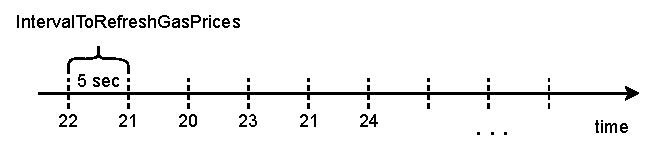
\includegraphics[width=0.8\columnwidth]{\zkevmdir/figures/architecture/economics-users-fees/l1-gasprice-refresh.drawio}
\end{figure}

In the example, we poll for the L1 gasPrice every 5 seconds and, as shown, gas prices vary with time.

In the following sections, we will thoroughly examine the significance of fees in Layer 2 and provide detailed answers to the previously mentioned questions.

We will focus first on the first part of the flow: \textbf{the RPC transaction pre-execution.}

\begin{figure}[H]
\centering
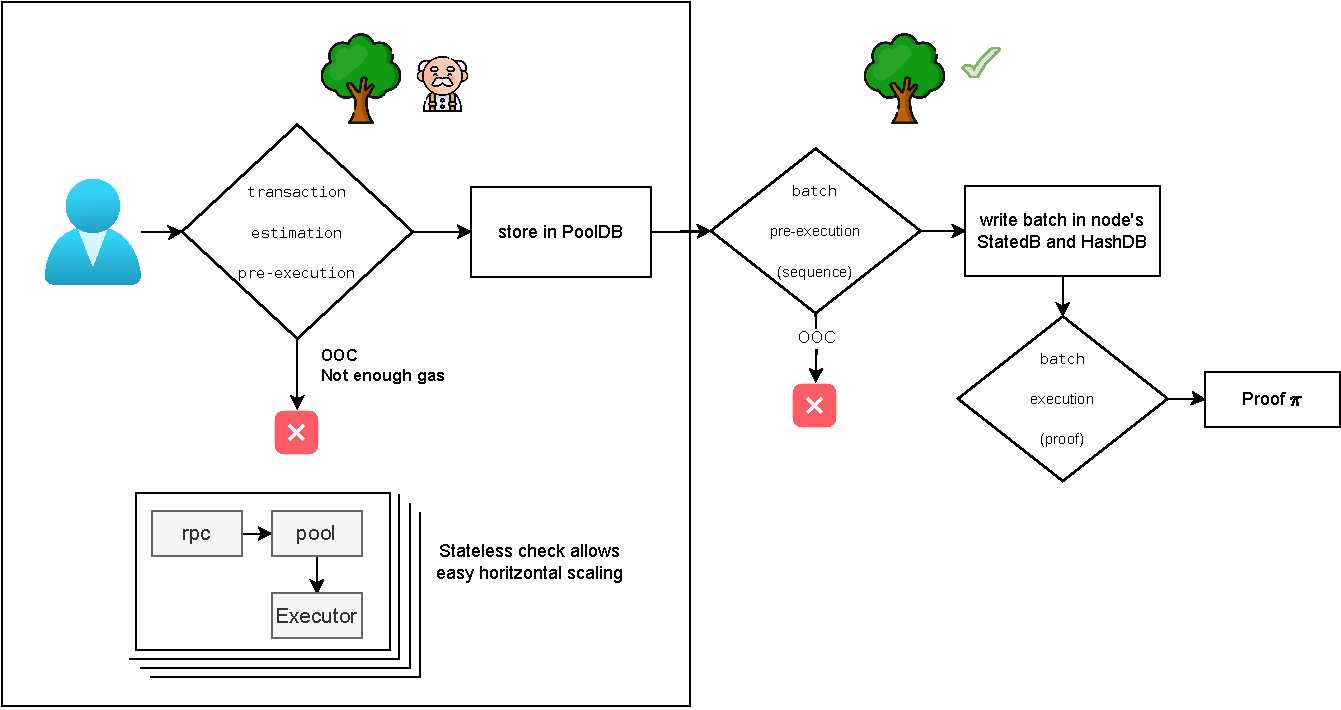
\includegraphics[width=0.8\columnwidth]{\zkevmdir/figures/architecture/economics-users-fees/rpc-preexecution.drawio}
\end{figure}


\section{Sending a Transaction}

This process is divided in two steps: \texttt{gasPrice} suggestion and sending the transaction.

\begin{enumerate}
\item \texttt{gasPrice} suggestion: the user asks via a RPC call for a suggested \texttt{gasPrice}. It is computed the following way:
\[
\texttt{L2GasPrice} = \texttt{L1GasPrice} \cdot \texttt{L1GasPriceFactor}
\]
to get an idea of a price to sign the transaction.
\begin{figure}[H]
\centering
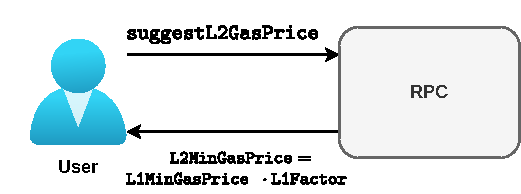
\includegraphics[scale=0.7]{\zkevmdir/figures/architecture/economics-users-fees/suggest-gasprice.drawio}
\end{figure}
\item Transaction sending: the user sends the desired L2 transaction with the decided \texttt{gasPrice}.
\begin{figure}[H]
\centering
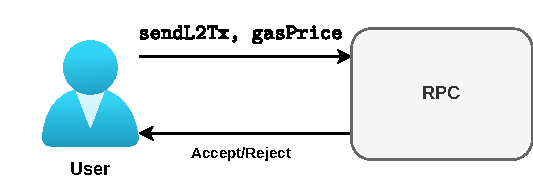
\includegraphics[scale=0.7]{\zkevmdir/figures/architecture/economics-users-fees/send-l2-tx-gasprice.drawio}
\end{figure}
\end{enumerate}

In case the \texttt{gasPrice} decided by the user is less than the current \texttt{L2GasPrice}, the transaction is automatically rejected and not included into the pool. This error is named \texttt{ErrGasPrice}.

The previous framework has a limitation as there is a time gap between step one and step two during which the gas price can fluctuate. This leads to the following unwanted situation:
\begin{figure}[H]
\centering
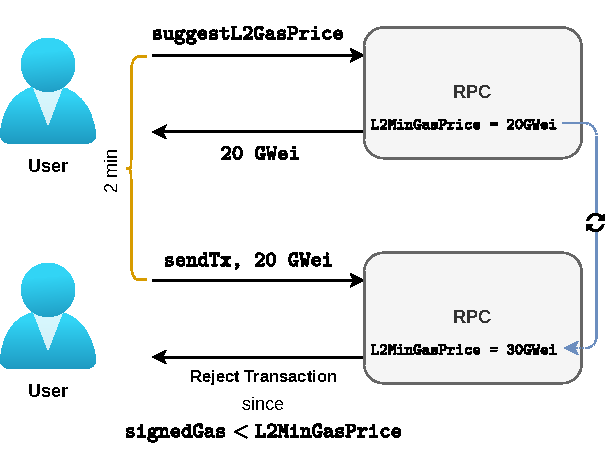
\includegraphics[scale=0.7]{\zkevmdir/figures/architecture/economics-users-fees/fees-bad-ux.drawio}
\end{figure}

In the previous figure we can observe that although the user has sent a \texttt{gasPrice} according to the suggested price, after the time lapse between one step and the other, the price has increased and the transaction is rejected.


The solution is to allow transactions from users that have signed any \texttt{SignedGasPrice} that is above the minumum L2 gas price recorded during a period of time called \texttt{MinAllowedPriceInterval}. This minimum price is denoted as \texttt{L2MinGasPrice}.

\begin{figure}[H]
\centering
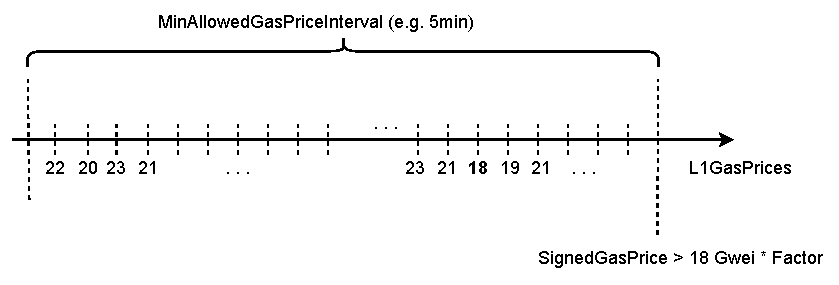
\includegraphics[scale=0.7]{\zkevmdir/figures/architecture/economics-users-fees/min-allowed-price-interval.drawio}
\end{figure}

This previous parameters can be configured in the Polygon zkEVM node:

%\begin{toml}
%[Pool]
%...
%DefaultMinGasPriceAllowed = 0
%MinAllowedGasPriceInterval = "5m"
%PollMinAllowedGasPriceInterval = "1s"
%IntervalToRefreshGasPrices = "5s"
%...
%\end{toml}
%\tiny
%\url{https://github.com/0xPolygonHermez/zkevm-node/blob/develop/docs/config-file/node-config-doc.md\#75-pooldb}
%
%\begin{itemize}
%\item \texttt{DefaultMinGasPriceAllowed:} It is the default min gas price to suggest.
%\item \texttt{MinAllowedGasPriceInterval:} It is the interval to look back of the suggested min gas price for a transaction.
%\item \texttt{PollMinAllowedGasPriceInterval:} It is the interval to poll L1 to find the suggested L2 min gas price.
%\item \texttt{IntervalToRefreshGasPrices:} It is the interval to refresh L2 gas prices.
%\end{itemize}
%
%When computing the L1 \texttt{gasPrice}, we can activate the \texttt{multigasprovider}:
%\begin{toml}
%[Etherman]
%...MultiGasProvider = false
%\end{toml}
%When enabled, it allows using multiples sources for computing the L1 \texttt{gasPrice}.


However, with this particular design, the zkEVM endpoint that provides a suggestion for the gas price that the user has to sign with its transaction (which will be called L2 Gas Price Suggester) has a \textbf{big problem design.} Recall that the price of posting transactional data to L1 is charged to the zkEVM network to the \textbf{full L1 price}. Therefore, if we propose a gas price using \texttt{L1GasPriceFactor}, representing the measure of computational reduction in L2, there is a risk of running out of Wei reserves for posting data to L1.  Consequently, we will recommend a slightly higher percentage of the gas price to the user, employing a \texttt{SuggesterFactor} of $0.15 \approx 4 \cdot \texttt{L1GasPriceFactor}$:
\[
\texttt{GasPriceSuggested} = \texttt{L1GasPrice} \cdot \texttt{SuggestedFactor}.
\]

Let's see a numerical example of how is the \texttt{GasPriceSuggested} computed:
\begin{figure}[H]
\centering
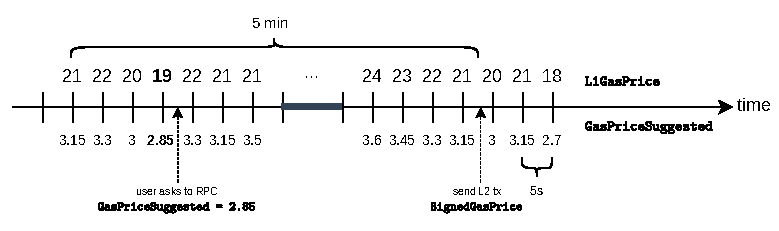
\includegraphics[scale=0.7]{\zkevmdir/figures/architecture/economics-users-fees/example-minimum-gas-price.drawio}
\end{figure}

When the user queries the suggested gas price through the RPC, the networks responds the current suggested gas price computed as $0.15 \cdot 19$, which is the current L1 gas price updated every $5$ seconds. However, at the time of sending the transaction, the RPC will only accept the transaction if $\texttt{GasPriceSigned}$ is strictly higher than the minimum suggested gas price from $5$ minutes ago (highlighted in \textbf{bold} in the figure), which in this instance is $19 \cdot 0.15 = 2.85$. In order to get his transaction accepted, the user sets the gas price of the transaction to $\texttt{GasPriceSigned} = 3.3 > 2.85 = \texttt{L2MinGasPrice}.$ The user has signed at a higher \texttt{gasPrice} than the suggested to ensure that the transaction is executed.




\section{Cost issues and strategies L1/L2}


In Ethereum, gas accounts for the resources used by a transaction, considering two elements in particular: \textbf{Data availability} (transaction bytes) and \textbf{Processing resources} like CPU, memory, and storage. Ethereum users commonly prioritize their transactions by increasing the \texttt{gasPrice}. A notable challenge arises when certain operations consume low gas in Layer 1 but represent a significant cost in Layer 2.

The costs associated with data availability are fixed once the transaction is known, and they are directly proportional to L1 data availability costs. On the other hand, L2 execution costs are variable, depending on the state, and typically offer a smaller cost per gas. Consequently, in our pricing schema, L2 transactions with high data availability costs and small execution costs are a significant challenge.

Recall that the Ethereum fee is computed as $\texttt{gasUsed} \cdot \texttt{gasPrice}$, giving us two ways of solving the misalignment problem when certain operations consume low gas in L1 but represent a significant cost in L2:

\begin{enumerate}[(A)]
\item \textbf{Arbitrum Approach. Increase \texttt{gasUsed}. }
This approach involves modifying the gas schema to elevate the Gas costs associated with data availability. While this strategy is relatively straightforward to implement and comprehend, it comes with a notable implication: \textbf{it changes the Ethereum protocol}. An L1 Ethereum transaction may execute different when compared to the same transaction executed in L2.
	
\item \textbf{Effective Gas Price Approach. Increase \texttt{gasPrice}. }
If we aim to avoid modifying the gas, the alternative is to increase the \texttt{gasPrice} to cover the costs. Unlike the previous approach, this doesn't alter the Ethereum specifications. However, determining a fair \texttt{gasPrice} becomes a complex task.  Moreover, we have to take into account that L2 users should be able to prioritize its transactions also increasing \texttt{gasPrice}, as they are used to. This is actually our approach.
\end{enumerate}


We will now develop how the \textbf{Effective Gas Price Approach} works. 

First, the user signs a relatively high gas price (\texttt{GasPriceSigned}) at the time of sending the L2 transaction. Later on, by pre-executing the sent transaction, the \textbf{sequencer} establishes a fair \texttt{gasPrice} according to the amount of resources used. To do so, the \textbf{sequencer} provides a single byte $\texttt{EffectivePercentageByte} \in \{0, 1, \dots, 255 \}$ (1 Byte), which will be used to compute a ratio called \texttt{effectivePercentage}:
\[
\texttt{EffectivePercentage} = \frac{1 + \texttt{EffectivePercentageByte}}{256}.
\]

This percentage will be used in order to compute the factor of the signed transaction's \texttt{gasPrice} which should be charged to the user %(or refunded)???:
\[
\texttt{TxGasPrice} = \left\lfloor \texttt{GasPriceSigned} \cdot \frac{1 + \texttt{EffectivePercentageByte}}{256} \right\rfloor.
\]

For example, setting an \texttt{EffectivePercentageByte} of $255 = \texttt{0xFF}$ would mean that the user would pay the totality of the \texttt{gasPrice} signed when sending the transaction:
\[
\texttt{TxGasPrice} = \texttt{GasPriceSigned}.
\]

In contrast, setting \texttt{EffectivePercentageByte} to $127$ would reduce the \texttt{gasPrice} signed by the user to the half:
\[
\texttt{TxGasPrice} = \frac{\texttt{GasPriceSigned}}{2}.
\]

In this schema, users \textbf{must trust the sequencer}. 

As having \texttt{EffectivePercentage} implies having \texttt{EffectivePercentageByte}, and vice versa, we will abuse of notation and use them interchangeably as \texttt{EffectivePercentage}.

To calculate the \texttt{EffectivePercentage}, one option is to consider the pricing resources based on the number of \textbf{consumed counters} within our proving system. However, understanding this metric can be challenging for users because stating the efficiency trough counters is not intuitive at the time of prioritizing their transactions. As we want to prioritize a positive user experience, we will consider an alternative where gas is used for calculations, as it is more user-friendly. So, our primary objective is to compute \texttt{EffectivePercentage} exclusively using Gas, allowing users to prioritize their transactions through the use of \texttt{gasPrice} without the need for intricate counter-based considerations.




\section{Introducing \texttt{BreakEvenGasPrice}}

As service providers, our primary goal is to \textbf{avoid accepting transactions that result in financial losses}. To attain this objective, we will determine the \texttt{BreakEvenGasPrice}, representing the lowest gas price at which we do not incur losses. As explained before, we will split the computation in two to take into account differently costs associated with data availability and costs associated with used Gas.


\subsection{Costs Associated with Data Availability}

Costs associated with Data Availability will be computed as
\[
\texttt{DataCost} \cdot \texttt{L1GasPrice},
\]
where \texttt{dataCost} is the cost in Gas for data in L1.

In the Ethereum ecosystem, the cost of data varies depending on whether it involves zero bytes or non-zero bytes. In particular, \textbf{non-zero bytes} cost \textbf{$16$ Gas} meanwhile \textbf{zero bytes} \textbf{$4$ Gas}.

Also recall that, when computing non-zero bytes cost we should take into account some constant data always appearing in a transaction: the \textbf{signature}, consisting on $65$ bytes and the \textbf{EffectivePercentageBytesLength}, consisting on $1$ byte related to the RLP-encoded fields length. This results in a total of $66$ constantly present bytes.

Taking all in consideration, \texttt{DataCost} can be computed as:
\[
(\texttt{TxConstBytes} + \texttt{TxNonZeroBytes}) \cdot \texttt{NonZeroByteGasCost} + \texttt{TxZeroBytes} \cdot \texttt{ZerByteGasCost},
\]
where \texttt{TxZeroBytes} (resp. \texttt{TxNonZeroBytes}) represents the count of zero bytes (resp. non-zero bytes) in the raw transaction sent by the user.


\subsection{Computational Costs}

For the computational cost, we will simply use the following formula:
\[
\texttt{GasUsed} \cdot \texttt{L2GasPrice},
\]
where recall that we can obtain \texttt{L2GasPrice} by multiplying \texttt{L1GasPrice} by chosen factor less than $1$:
\[
\texttt{L2GasPrice} = \texttt{L1GasPrice} \cdot \texttt{L1GasPriceFactor}.
\]
In particular, we will choose a factor of $0.04$.

In contrast to data availability costs, to compute computational costs we will need to \textbf{execute} the transaction.

%TODO separar

Combining both \textbf{data} and \textbf{computational} costs, we will refer to it as \texttt{TotalTxPrice}:
\[
\texttt{TotalTxPrice} = \texttt{DataCost} \cdot \texttt{L1GasPrice} + \texttt{GasUsed} \cdot \texttt{L1GasPrice} \cdot \texttt{L1GasPriceFactor}.
\]

To establish the gas price at which the total transaction cost is covered we can compute \texttt{BreakEvenGasPrice} as the following ratio:
\[
\texttt{BreakEvenGasPrice} = \frac{\texttt{TotalTxPrice}}{\texttt{GasUsed}}.
\]
Additionally, we incorporate a factor $\texttt{NetProfit} \geq 1$ that allows us to achieve a slight profit margin:
\[
\texttt{BreakEvenGasPrice} = \frac{\texttt{TotalTxPrice}}{\texttt{GasUsed}} \cdot \texttt{NetProfit}.
\]

Observe that we still need to introduce here \texttt{gasPrice} prioritization, which will be covered later on.


\subsection{Numerical Examples}

\begin{enumerate}

\item About how to calculate the \texttt{BreakEvenGasPrice}:

Recall the example proposed before, where the user ended up by setting \texttt{GasPriceSigned} to $2.85$. Suppose the user sends a transaction having: $200$ non-zero bytes, including the constant ones and $100$ zero bytes. Moreover, at the time of pre-executing the transaction (without getting an \textbf{OOC} error), $60,000$ Gas is consumed (recall that, since we are using a \textit{wrong} state root, this gas is only an estimation).

\begin{figure}[H]
\centering
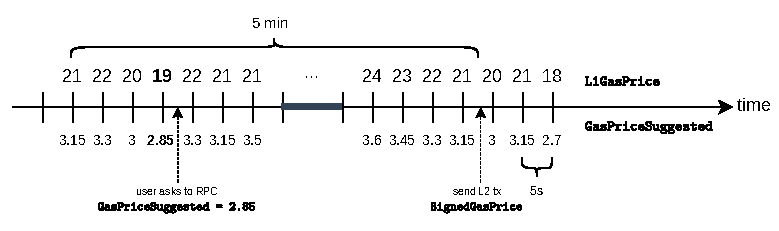
\includegraphics[scale=0.9]{\zkevmdir/figures/architecture/economics-users-fees/example-minimum-gas-price.drawio}
\end{figure}

Hence, following the formulas previously explained, the total transaction cost is of
\[
\left( 200 \cdot 16 + 100 \cdot 4 \right) \cdot 21 + 60,000 \cdot 21 \cdot 0.04 = 126,000 \text{ GWei}.
\]

Observe that $21$ is the \texttt{L1GasPrice} at the time of sending the transaction.

Now, we are able to compute the \texttt{BreakEvenGasPrice} as
\[
\texttt{BreakEvenGasPrice} = \frac{\texttt{TotalTxPrice}}{\texttt{GasUsed}} = \frac{126,000 \text{ GWei}}{60,000 \text{ Gas}} \cdot 1,2 = 2.52 \text{ GWei/Gas}.
\]

We have introduced a \texttt{NetProfit} value of $1.2$, indicating a target of a $20\%$ gain in this process.

At a first glance, we might conclude acceptance since $\texttt{GasPriceSigned} = 3.3 > 2.52$ but, recall that this is only an estimation, gas consumed with the correct state root can differ. To avoid this issue, we introduce a \texttt{BreakEvenFactor} of $30\%$ to account for estimation uncertainties:
\[
\texttt{GasPriceSigned} = 3.3 > 3.276 = 2.52 \cdot 1.3 = \texttt{BreakEvenGasPrice} \cdot \texttt{BreakEvenFactor}.
\]

Consequently, we decide to \textbf{accept the transaction}.



\item About how to calculate the \texttt{BreakEvenFactor}:

Imagine we disable the \texttt{BreakEvenFactor} setting it to $1$. Our original transaction's pre-execution consumed $60$k Gas, $\texttt{GasUsedRPC} = 60$k. However, imagine that the correct execution at the time of sequencing consumes $35$k Gas. If we recompute \texttt{BreakEvenGasPrice} using this updated used gas, we get $3.6 \text{ GWei/Gas}$, which is way higher than the original one. That means that, we should have charged the user with a higher gas price in order to cover the whole transaction cost, which now is of $105,000$ GWei.

But, since we are accepting all the transactions signing more than $2.85$ of gas price, we do not have margin to increase more. In the worst case we are loosing
\[
105,000 - 35,000 \cdot 2.85 = 5,250 \text{ GWei}.
\]

Introducing \texttt{BreakEvenFactor} we are limiting the accepted transactions to the ones having
\[
\texttt{GasPriceSigned} \geq 3.27,
\]
in order to compensate such losses.

In this case, we have the flexibility to avoid losses and adjust both user and our benefits since
\[
105,000 - 35,000 \cdot 3.27 < 0.
\]

\textbf{Final Note}:  In the example, even though we assumed that the decrease in \texttt{BreakEvenGasPrice} is a result of executing with a correct state root, it can also decrease significantly due to a substantial reduction in \texttt{L1GasPrice}.
\end{enumerate}



\section{Introducing Priority}

Prioritization of transactions in Ethereum is determined by \texttt{GasPriceSigned}: transactions signed at a higher price will be given priority. To implement this, consider that users are only aware of two gas price values: the one signed with the transaction, called \texttt{GasPriceSigned} and the current \texttt{GasPriceSuggested}, which is the one that provides the RPC.

At the time of sequencing a transaction, we should prioritize ones among the others, depending basically on both \texttt{GasPriceSigned} and current \texttt{GasPriceSuggested}. In the case that $\texttt{GasPriceSigned} > \texttt{GasPriceSuggested}$, we establish a priority ratio as follows:
\[
\texttt{PriorityRatio} = \frac{\texttt{GasPriceSigned}}{\texttt{GasPriceSuggested}} - 1.
\]

If $\texttt{GasPriceSigned} \leq \texttt{GasPriceSuggested}$, the user has chosen not to proritize its transaction (and maybe we can reject the transaction due to low gas price). In this case, we establish a priority ratio to be $0$.

The \texttt{EffectiveGasPrice} will be computed as:
\[
\texttt{EffectiveGasPrice} = \texttt{BreakEvenGasPrice} \cdot (1 + \texttt{PriorityRatio}).
\]


Let's see it with an example:

Recall that, in the previous example, we were signing a gas price of $3.3$ at the time of sending the transaction. Suppose that, at the time of sequencing a transaction, the suggested gas price is 3.
\[
\texttt{GasPriceSuggested} = 3.
\]
The difference between both is taken into account in the priority ratio:
\[
\texttt{PriorityRatio} = \frac{3.3}{3} - 1 = 0.1.
\]
Henceforth, the estimated \texttt{EffectiveGasPrice} (that is, the one using the RPC gas usage estimations) will be
\[
\texttt{EffectiveGasPrice} = 2.52 \cdot (1 + 0.1) = 2.772.
\]
